\chapter{Static digitalization of society}

\section{OpenStreetMap}

\begin{figure}[h]
  \centering
  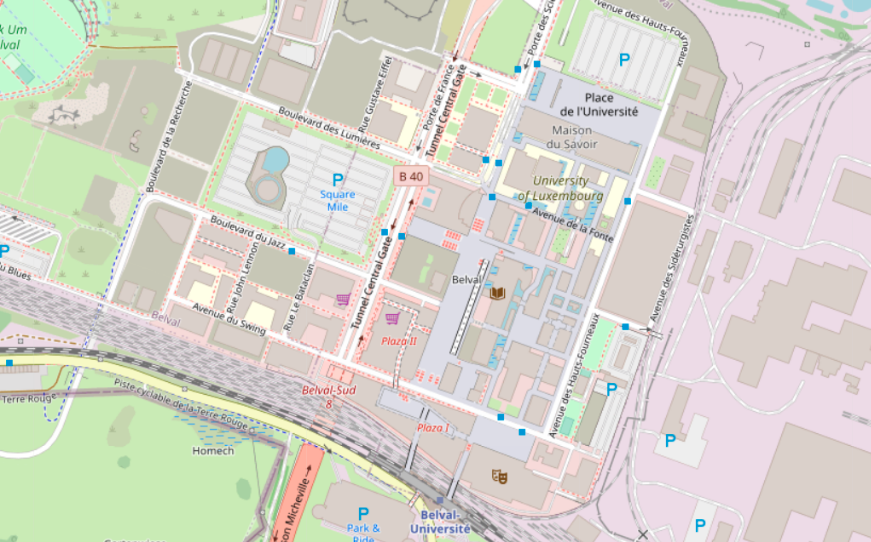
\includegraphics[width=0.8\linewidth]{Media/BelvalOSM.png}
  \caption{\centering {\small A cartographic overview of the Belval campus in openstreetmap format.}}
  \label{fig:belvalosm}
\end{figure}

To design a static digitalization of society as authentic as possible, the project bases its design on the use of an \textit{openstreetmap} file of the territory studied. Everything starts from this starting point. The idea is to use the places and the real road network of a determined area to initialize the locations, and have the support of paths between the different places.\\

To facilitate the execution of the project, it is therefore interesting to be able to retrieve the \textit{openstreetmap} file directly from the program. To do this, we fill in several information such as the bounds representing the minimum and maximum latitudes and longitudes in a Python implementation named \textit{Overpy}.\\

One of the small disadvantages of \textit{openstreetmap} is the delimitation of the territory studied. Beforehand, it is possible to recover a region by forming a polygon, most often rectangular but it is not intuitive in our use here. In particular to use demographic statistics for example, which are appropriate for a certain delimitation of a territory. It would be necessary to check the possible filters already existing before deepening this approach but it seems wise to transform the recovered file by filtering the elements that are contained within a well-defined perimeter : we can speak of ``administrative'' limits of the territories where we look at the official borders between the different regions. In general, it would be very interesting to evaluate the position of the elements in relation to a peripheral boundary. If there is no attribute in the element that indicates its administrative location, it would be necessary to model the delimitation by a sequence of points with acceptable longitudes and latitudes to check element by element. There are probably already algorithms for this filtration.\\

Another interesting point to look at is the proximity of an element to the boundaries of the territory. This is already more complex than knowing if the element is contained within the perimeter and therefore requires a little more work. An element located near a border may have a different treatment in digitalization but we will see this point a little later.\\

In a later version, it might be interesting to see an interest in breaking down a large geographical area into a mosaic of several small areas in order to parallelize the static digitalization of society.\\

\newpage

\section{Places}

\subsection{Format openstreetmap}

Initially described by an \textit{openstreetmap} file, places have characteristics specific to the file format. It is therefore necessary to read all the elements and rework the characteristics of each of the places. A location is primarily described by a set of nodes, each of which has a precise latitude and longitude. This set of nodes forms an enclosed place that delineates the contours of each place. By simply reworking the data, each place can be characterized by common attributes : \\

\begin{itemize}
\item A unique identifier, taken from the \textit{osm} file.
\item Nodes that delimit it ; useless in a simple version but which may possibly be of perfectionist interest.
\item Its average location, calculated with the average of its nodes ; the result is questionable in geometric terms but sufficient to summarize the position of the place.
\item Its area, calculated with its nodes ; calculating an area of any polygon with geographic coordinates is very imperfect and requires the use of the \textit{Shapely} package.
\item Labels from the original file that can provide realistic specifications to spaces ; we will find the original classification of the place in \textit{openstreetmap} and sometimes amusing information such as the name of the structure, etc.\\
\end{itemize}


The following link provides more information about the \textit{openstreetmap} format : \href{https://wiki.openstreetmap.org/wiki/FR:\%C3\%89l\%C3\%A9ments\_cartographiques}{\textit{Wiki OpenStreetMap}}\\

\subsection{Database}

The reading of the elements in the file is sequential and can not be parallelized beforehand. The file structure is broken down into nodes, path, and relationship, preventing independent processing of subsets of the file. However, as mentioned above, it is possible with a pre-processing step for geographical import to divide the territory into several sub-territories to read them independently.\\

It is obvious to register the places in a database for the use of digitalization. Instead of simply saving the interesting elements of the file, it is therefore advisable to think about the memory management of these locations.\\

In the \textit{openstreetmap} format, places are classified according to a key and a value according to the type of location. To best digitize an epidemic, the implementation reclassified the different types of places in order to better group locations according to their societal role, their economic function or their ability to accentuate the contamination of their occupants. The underlying idea is to treat places of the same category with common parameters. The new classification is described by types, which in turn consist of subtypes. The role of room types is more affiliated with a consistent organization of the database. They mainly allow subtypes to be logically grouped together, which can be useful for example to treat subtypes in the same way.\\

Each subtype therefore has common characteristics that allow, for example, to adjust the health and economic evaluations of each places associated with them. These parameters make it possible to adapt the value returned by the sanitary and economic functions of the locations. \\

\subsection{Advanced attributes}

Common attributes can easily be added to places, subtypes, or even to the types of locations themselves. In most cases, it is best to define attributes in subtypes by a Python dictionary. Their uses in practice can be modulated by means the simple attributes of places such as area. This is the case, for example, with assessment factors relating to the economy or health risks. After that, we can specify the subtypes more by reducing the roles that their places can play. The explanation of the roles will be given with dynamic digitalization.\\

In terms of attributes, we can extend the prospects of evolution by adding, for example :\\

\begin{itemize}
\item Opening and closing times ; these schedules must be acceptable and logical in relation to the categories of spaces.
\item Average passage time of individuals ; to nuance with random parameters and by dissociating the different roles of individuals.
\item Obligation to present a valid known condition ; depending on health validity or other tests.
\item Possibility of teleworking and the associated percentage of performance ; only working hours are considered in economic terms and this parameter is therefore exclusive to places with a work role.
\item Limit of the occupants at the same time ; by not considering individuals with the role of workers and by nuance with the area of locations.\\
\end{itemize}

\subsection{Distance management}

\begin{wrapfigure}{l}{0.25\linewidth}
  \centering
  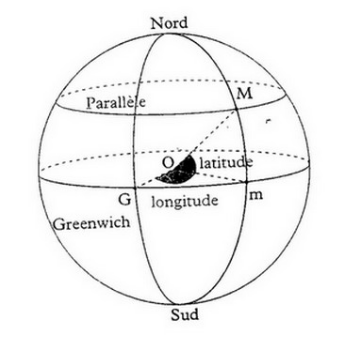
\includegraphics[width=\linewidth]{Media/Geographie.png}
\end{wrapfigure}

In modeling, places make it possible to add
distance design to the digitalization of society. However, all geographic data are given in latitude and longitude. There are two ways to calculate the metric from this data. There is a \textit{Shapely} package in Python that allows you to have accurate results but takes longer to execute compared to the simple mathematical method. \textit{Shapely} is therefore applied to obtain exact results to record such as the area of places. It is preferable to use the simple method to compare distances. This is the case, for example, to select the nearest place from a location. We can also filter a set of places according to their relative distance to a location, but also according to their area or category. Due to some uncertainty, the results may differ significantly from the \textit{Shapely} long method. It will therefore be necessary to empirically add a factor to the mathematical method to adjust it to the long one.\\

\newpage

\section{Individuals}

\subsection{Constitution of static data}

The use of cartographic data from an \textit{openstreetmap} file does not make it possible to constitute the demographic heritage of a territory. It is necessary to find strategies to identify the number of individuals to initialize as well as to characterize them adequately.\\

The best method is to combine the delimitation of an \textit{openstreetmap} territory with the administrative boundaries of a region in order to make the best use of local demographic data. If this is not possible, then we can analyze the \textit{openstreetmap} file itself and find solid correlations between the number of individuals and elements of the file. For example, a linear regression between the total file size and the population of the region could be sought. Otherwise, by analyzing in more detail, we can look at the total area of accommodations in the file to deduce the number of individuals. There are many possible hypotheses just waiting to be tested. Of course, it is always possible to define a number of individuals manually, independently of the map data.\\

In our case of the internship, the Grand Duchy of Luxembourg provides a very interesting set of public data on a website : 
\href{https://data.public.lu/fr/ }{\textit{Public Data of Luxembourg}}\\


In the case of this section, this concerns demographic data or household data for example. To best represent the population in this project, we therefore have the total population by Luxembourg region in 2021.\\

\subsection{Representation of individual diversity}

How to bring the static diversity of individuals ?\\

Especially in the context of an epidemic study, it is necessary to be able to represent the diversity of organisms in terms of resistance, fragility, etc. And from the simple point of view of society, it is essential to distinguish individuals with significantly different dynamics. For example, students will not have the same dynamic as retirees.\\

However, we can find a common factor rather simple : age. By nuanced with classes of individuals with similar behaviors, it seems intuitive to characterize an individual by age and socio-dynamic category.\\

It is also available to know the distribution of the Luxembourg population according to age, from 0 to 95 years. For the sake of simplicity, the proportion of the Luxembourg population over 95 is added to the initialization. The current population of the implementation is therefore divided between 0 and 95 years. Beforehand, it seems unproductive to focus on the evolution of population ages, births and non-infectious mortalities. But we can nevertheless leave the door open to these avenues of exploration for other benevolent projects concerning demographic change, for example.\\

\subsection{Database}

Like places, individuals are classified into types and subtypes. We find the principle of dictionary to list common characteristics.\\

A subtype of individuals has several basic attributes :\\

\begin{itemize}
\item  The minimum age and maximum age of the individuals who compose it.
\item The categories of accommodations in which its individuals can sleep.
\item The categories of places in which its individuals can work.\\
\end{itemize}

On the side of individuals, each of them would be characterized by :\\

\begin{itemize}
\item A unique identifier.
\item An age.
\item A set of data corresponding to the personal base.\\
\end{itemize}

How to distribute the ages of individuals in digitalization ?\\

It is an ambiguous problem. On the one hand we have the socio-dynamic classes of individuals and on the other the age distribution of a territory. We can question the choices of implementation but the chosen solution seems appropriate at first :\\

At initialization, the total number of individuals is arbitrarily distributed across all existing types of the database. We therefore have a subnumber of individuals to distribute between the different subtypes in each of the types. This is where the age distribution of the territory, in this case Luxembourg, is used. Only the age range identified in the subtype is taken and the proportions are determined relative to a total of 100\%.\\

In the case of a tangled set of subtypes with overlapping age intervals, it is preferable to respect the distribution of the territory over the entire type of individuals. As a result, all the age intervals of the subtypes are first recovered in the same interval, re-proportioned on a scale of 100\%. The initialization begins by choosing an age respecting the different probabilities of each of them. When the selected age can be associated with several categories, the choice of subtype is then made randomly with equiprobability.\\

The demographic distribution of ages is therefore respected at the level of a type, but important nuances can be found when considering a set of types of individuals. It is even possible not to find certain age ranges in static digitization.\\

\subsection{External consideration}

One of the great complexities in digitalization, whether static or dynamic, is the external modeling of the territory. All territories are permeable, unless we take
the world as a whole, which is unthinkable. However, it would be interesting to discuss the correlation between the surface of the territory studied and the static, and dynamic, outdoor affluence to be digitized. For the same surface, we will find an external influence much greater in Paris than in a countryside. So is there rather a correlation with the ``internal'' population of the territory, which as a reminder can also be estimated from the \textit{openstreetmap} file itself ?\\

Now, it is true that we can question the relevance of age and socio-dynamic classes. Are the ``external'' individuals always the same ? As a whole, do we find a distribution of ages that is logical or similar to the territory studied ? Is there even an interest in recording them, or rather representing them by spontaneous individuals with random attributes ?\\

It is obvious that this approach must be deepened with more hindsights and reflections. From a static point of view, external persons can be identified by their occupation with the role of worker ; the distinction between interns and externals is based on the position of their home in relation to the territory. And then from a dynamic view, we must also add individuals a little randomly, with a frequency and diversity to discuss.\\

Their digitization is essential but requires more reflections to talk about it.\\

\subsection{Individual base}

The individual base are essential assignments. They make it possible to bring a form of determinism and coherence in dynamic digitalization. In an initial version, the base is represented by the individual's housing place and work place. In both, it also seems sensible to specify the frequent local entourage of the individual. In absolute terms, this makes it possible to have a very good modeling of the digitalization of each individual in a case of great dynamic restriction.\\

In the case of the epidemic study, it is more than essential to have good modeling in case of major political restrictions. This would make it possible, for example, to see the real effectiveness of containment and to observe possible flaws in the connection of contact networks, for example.\\

Of course, this base can evolve over time but it is assumed that the individual keeps his home, his roommates, his work and his close colleagues in a first version. We will see later ways to add more information to model and anticipate the dynamic base of the individual. This will be the case, for example, with dynamic digitalization, where it will be important to assign a mode of transport to each individual. Among the most relevant tracks, we can be interested in considering the close friendships and family relationships of the individual. However, the question of the exploitation of this base in dynamic terms remains to be deepened. Similarly, we can possibly extend the base with the habits of individuals, which can be compared to needs more precisely here, such as the daily visit of the individual to a gym to cite an example. Playful habits would really not be relevant, or even interesting, to consider to simplify the design.\\

It should be noted that this conception does not consider the age of individuals : children are considered independent persons with housing, workplace, etc. In this case, care should be taken to establish a school as a workplace. We can then think about the workspace of individuals without work. Is it empty and in which case it would be necessary to treat this case separately, or should it be represented by their housing place ?\\

How to assign the individual's housing and work places ?\\

The objective is simple, to make a join between the database of internal individuals and that of housing places. As a reminder, each category of individual has a list of housing categories where he can reside. For example, retirement institutions will not be able to be found in a socio-dynamic category of children. This also leads to other reflections for the classification of categories of individuals to specifically associate disabled individuals with adequate housing establishments. The same principle is found at the level of professional places. Each category has defined sets. However, it is necessary to take into account the complexity of the professional distribution of a territory.\\

In a simple version, the selection is made randomly among the set of categories associated with it, excluding no place specifically. The adjustment is made by weighting the selection with the area of each locations. Therefore, a place with one area greater than another will have proportionally more assignment than the second. We can of course review this selection to perfect the static digitization of the observed data. Similarly, it might be wise to look at the possibility of excluding places in selections.\\

This conception is not complete : it is necessary to be able to identify the people really close to the individual in each of these key places. For example, when the location in question is a small apartment, all the individuals in the accommodation are indeed in contact. On the other hand, when the accommodation is a large residence as a whole, very few people are really in contact with the individual. This is why it is necessary to list the people to be close to the individual in each of the assigned places. The ideal would be to use real demographic data such as the distribution of the number of people in households. Indeed, this attribution is made iteratively, without wanting to reproduce logic in the construction of households. The program does not seek, for example, to gather two children and two adults in their forties. Therefore, it is totally possible to observe original groupings such as five children in a house. This problem of coherence has less impact on workplaces since there seems to be more heterogeneity. Especially since a certain logic is respected with the association of job categories with that of individuals. For instance, there is no risk of observing children, whose work is school, working alongside adults ; except when it comes to teachers. Of course, we can also look at the real data of the territory on the distribution of the labor market for more realism.

